
\documentclass{beamer}
\beamertemplatenavigationsymbolsempty
\graphicspath{ {./images/} }
\setbeamercolor{section number projected}{bg=red,fg=white}
\setbeamercolor{subsection number projected}{bg=red}
\setbeamertemplate{itemize items}[triangle]
\setbeamercolor{itemize item}{fg=red}
\setbeamertemplate{itemize subitem}[circle]
\setbeamercolor{itemize subitem}{fg=red}
\usepackage{multicol}

\mode<presentation>
{
  	\usetheme{CambridgeUS}
  	\setbeamercovered{transparent}
}

\usepackage[english]{babel}
\usepackage[utf8]{inputenc}
\usepackage{times}
\usepackage[T1]{fontenc}

\title[Face recognition]{\textbf{Multiple face recognition in images}}
\subtitle{\texttt{Presentation on Convolutional Neural Networks, 2018}}

\author[Simone Caldarella]
{Simone~Caldarella\\
s.caldarella@studenti.unibs.it}

\institute[University of Brescia] 
{
  	IEEE Student Branch Brescia\\
  	University of Brescia
}

\date[IEEE Student Branch 2018] 
{
	5/12/2018
}

\subject{Theoretical Computer Science}

\AtBeginSubsection[]
{
 	\begin{frame}<beamer>{Outline}
		\begin{multicols}{2}
			\setlength\itemsep{1em}
   			\tableofcontents[currentsection,currentsubsection]
		\end{multicols}
  	\end{frame}
}

\begin{document}

\begin{frame}
 	\titlepage
\end{frame}

\begin{frame}{Outline}
	\begin{multicols}{2}
  		\tableofcontents
	\end{multicols}
\end{frame}

%#####################################INTRODUCTION############################################################

\section{Introduction}

%\subsection{Motivation}

\begin{frame}{Motivation}
	\begin{itemize}
		\setlength\itemsep{1em}
		\setbeamertemplate{itemize items}[triangle]
		\setbeamercolor{itemize item}{fg=red}
		\item
			Machine learning is a field in continuos spreading.
		\item
			Problem: IEEE student branch's members' recognition using neural network.
		\item 
    			Create a ground for recognition problems.
		\item
			Goal: implementing a face recognition system for the student branch's members, expecially:
		\begin{itemize}
				\setbeamertemplate{itemize subitem}[circle]
				\setbeamercolor{itemize subitem}{fg=red}
    				\item
      					detect and recognize different faces in photos;
    				\item    
      					use a computer vision's framework (OpenCv) and a machine learning framework (Tensorflow).
 
			\end{itemize}
	\end{itemize}
\end{frame}


%#####################################BACKGROUND############################################################

\section{Background}

\subsection{Machine learning}

\begin{frame}{What does machine learning means?}
	\begin{itemize}
		\setbeamertemplate{itemize items}[triangle]
		\setbeamercolor{itemize item}{fg=red}
  		\item
    			Is this a \textbf{neural network} or a \textbf{graph}?
	\end{itemize}
	\begin{center}
		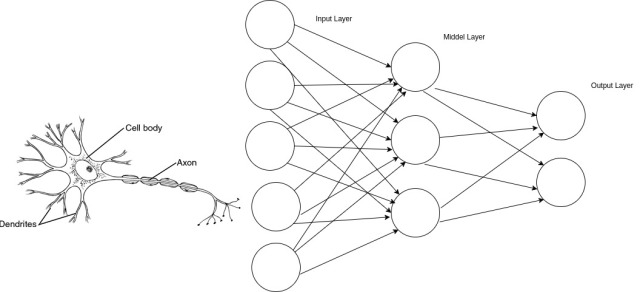
\includegraphics[scale=0.5]{neuralNet}
	\end{center}
\end{frame}

\begin{frame}{What does machine learning means?}
	\begin{itemize}
		\setlength\itemsep{1em}
		\setbeamertemplate{itemize item}[triangle]
		\setbeamercolor{itemize item}{fg=red}
  		\item 
			The concept of \textbf{training}:
    			\begin{itemize}
				\setbeamertemplate{itemize subitem}[circle]
				\setbeamercolor{itemize subitem}{fg=red}
    				\item
      					input and output;
    				\item    
      					inference and loss function;
   				\item
					gradient descent and weights update.
			\end{itemize}
		\item
    			The importance of a large and well structured dataset:
    			\begin{itemize}
				\setbeamertemplate{itemize subitem}[circle]
				\setbeamercolor{itemize subitem}{fg=red}
   				\item 
					common problems;
    				\item 
					cognitive bias.
    			\end{itemize}
 	 \end{itemize}
\end{frame}

\begin{frame}{Training and gradient descent}
	\begin{center}
    		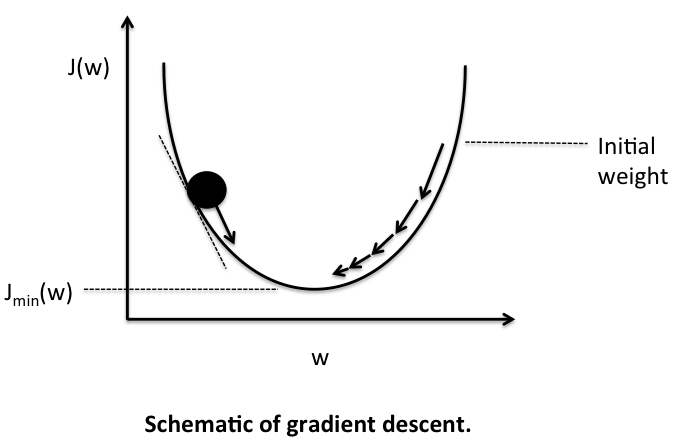
\includegraphics[scale=0.4]{grad}
	\end{center}
\end{frame}

\begin{frame}{A more complex gradient descent loss}
	\begin{center}
    		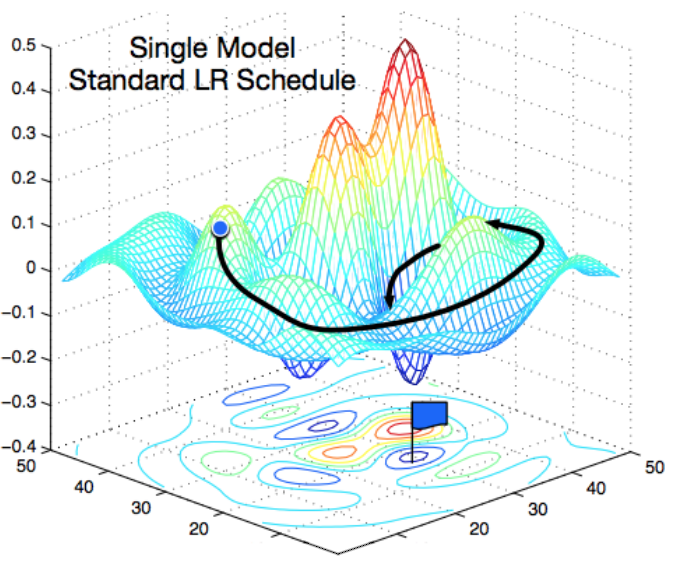
\includegraphics[scale=1.3]{suchcomp}
	\end{center}
\end{frame}

\subsection{Tensorflow and OpenCv}

\begin{frame}{Tensorflow and OpenCv}
	\begin{itemize}
		\setlength\itemsep{1em}
		\setbeamertemplate{itemize item}[triangle]
		\setbeamercolor{itemize item}{fg=red}
		\item 
			Tensorflow and computational graph concept
	\end{itemize}
	\begin{center}
    		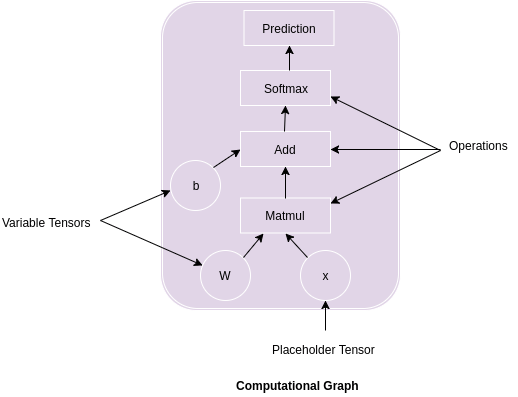
\includegraphics[scale=0.4]{comp}
	\end{center}
\end{frame}

\begin{frame}{Tensorflow}
	\begin{itemize}
		\setlength\itemsep{1em}
		\setbeamertemplate{itemize item}[triangle]
		\setbeamercolor{itemize item}{fg=red}
		\item
			Why Tensorflow?
			\begin{itemize}
				\setbeamertemplate{itemize subitem}[circle]
				\setbeamercolor{itemize subitem}{fg=red}
				\item 
					Tensors and use of computational graph;
				\item 
					different levels of abstraction.
			\end{itemize}
		\item 
			Low level and high level API:
			\begin{itemize}
				\setbeamertemplate{itemize subitem}[circle]
				\setbeamercolor{itemize subitem}{fg=red}
				\item 
					Tensorflow functions;
				\item 
					\texttt{Keras} and \texttt{tflearn}.
			\end{itemize}
	\end{itemize}
\end{frame}

\begin{frame}{OpenCV}
	\begin{itemize}
		\setlength\itemsep{1em}
		\setbeamertemplate{itemize item}[triangle]
		\setbeamercolor{itemize item}{fg=red}
		\item
			Why OpenCV?
			\begin{itemize}
				\setbeamertemplate{itemize subitem}[circle]
				\setbeamercolor{itemize subitem}{fg=red}
				\item 
					Very fast;
				\item 
					lots of library and algorithm at the state-of-art.
			\end{itemize}
		\item 
			OpenCV detection algorithm:
			\begin{itemize}
				\setbeamertemplate{itemize subitem}[circle]
				\setbeamercolor{itemize subitem}{fg=red}
				\item 
					\texttt{HaarCascadeClassifier};
				\item 
					\texttt{Dlib} library for face features detection.
			\end{itemize}
	\end{itemize}
\end{frame}



%\section{Image classification}

\subsection{Convolutional Neural Network}

\begin{frame}{Convolutional Neural Network (CNN)}
	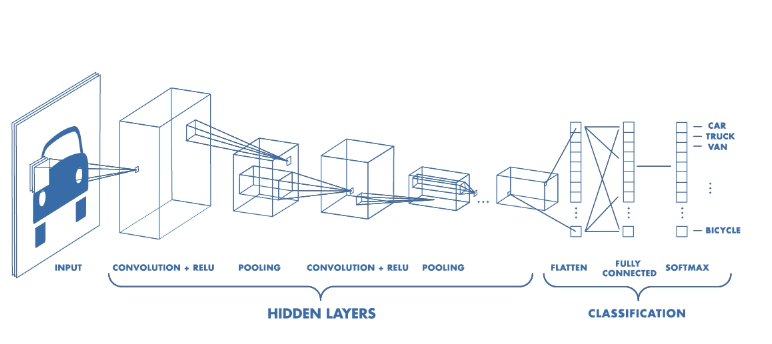
\includegraphics[scale=0.45]{CNN}
\end{frame}

\begin{frame}{Convolutional layers}
	\begin{itemize}
		\setlength\itemsep{1em}
		\setbeamertemplate{itemize item}[triangle]
		\setbeamercolor{itemize item}{fg=red}
		\item 
			Convolutional matrix (Kernel)
	\end{itemize}
	%\begin{center}
		%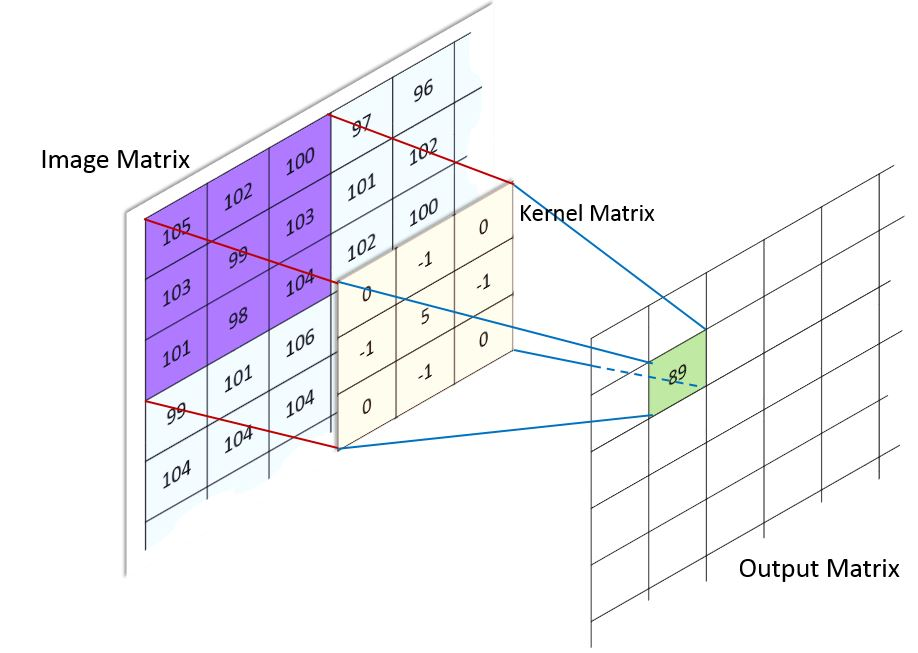
\includegraphics[scale=0.2]{kernel}
		%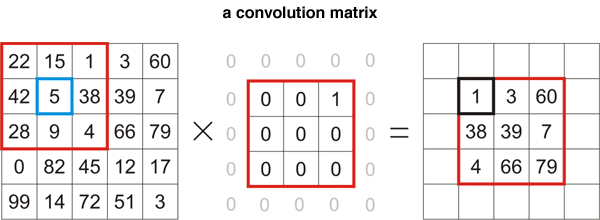
\includegraphics[scale=0.2]{conv}
	%\end{center}
	%\begin{figure}
		%\centering
		%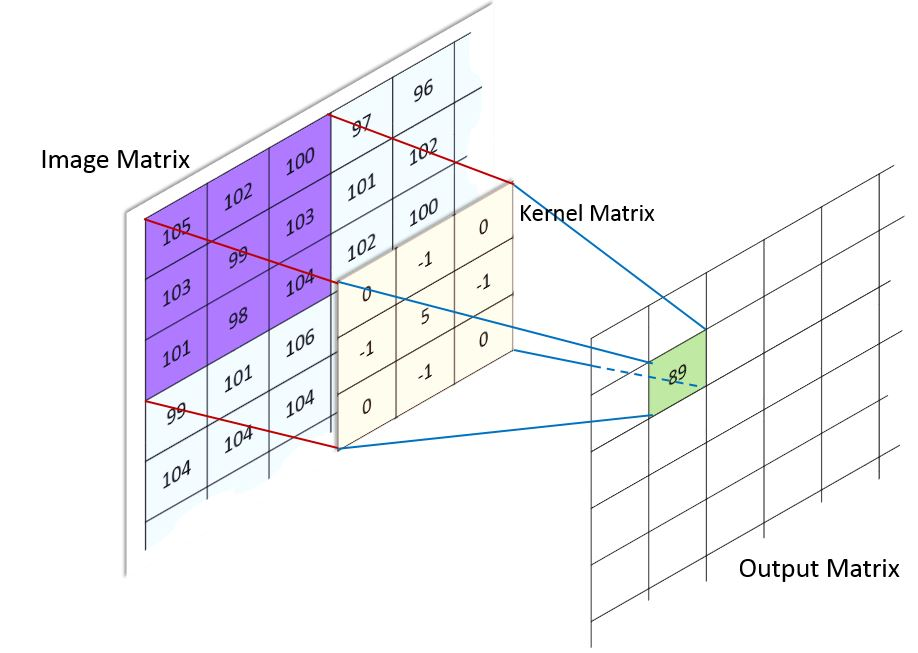
\includegraphics[width=.49\textwidth]{kernel}\hfil
		%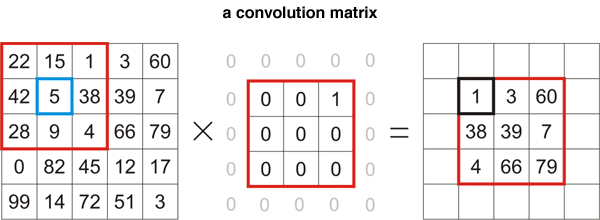
\includegraphics[width=.49\textwidth]{conv}
	%\end{figure}
	\begin{center}
	\begin{minipage}{6in}
  		%\centering
  			$\vcenter{\hbox{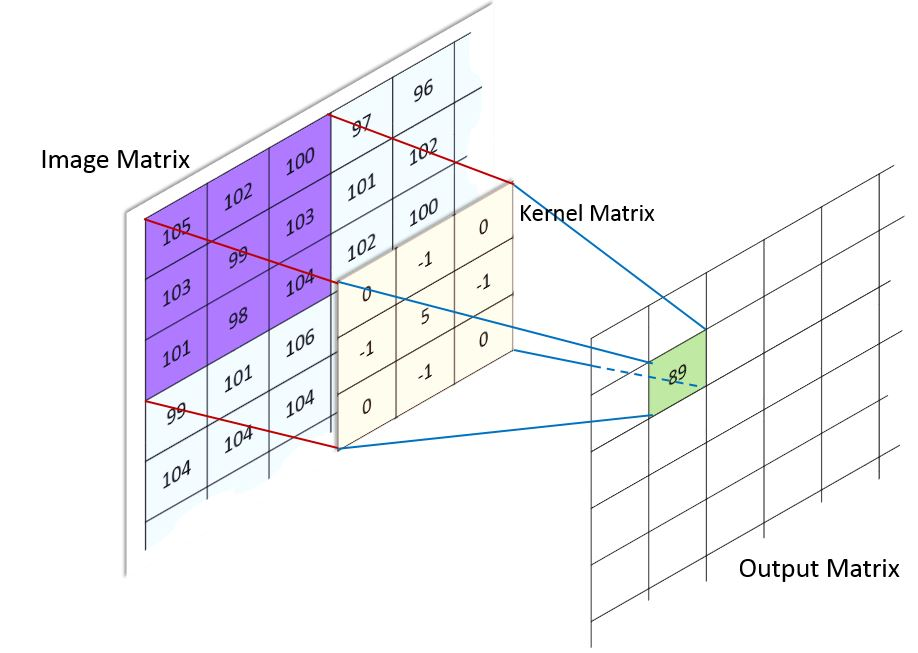
\includegraphics[scale=0.2]{kernel}}}$
 			 \hspace*{.2in}
  			$\vcenter{\hbox{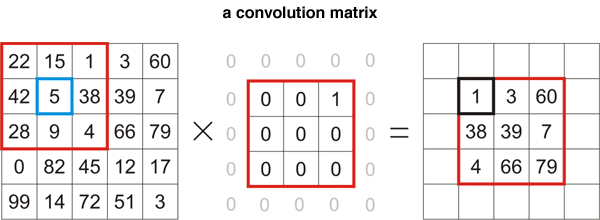
\includegraphics[scale=0.27]{conv}}}$
	\end{minipage}
	\end{center}
	\begin{itemize}
		\setlength\itemsep{1em}
		\setbeamertemplate{itemize item}[triangle]
		\setbeamercolor{itemize item}{fg=red}
		\item 
			3x3, 5x5, or 7x7, why only odd numbers?
		\item 
			Edge detection:
			\begin{itemize}
				\setbeamertemplate{itemize subitem}[circle]
				\setbeamercolor{itemize subitem}{fg=red}
				\item 
					Similarity with human vision;
				\item 
					From simple to complex forms.
			\end{itemize}
	\end{itemize}
\end{frame}

\begin{frame}{Pooling layers}
	\begin{itemize}
		\setlength\itemsep{1em}
		\setbeamertemplate{itemize item}[triangle]
		\setbeamercolor{itemize item}{fg=red}
		\item 
			Reducing number of information: best way to avoiding \textbf{overfitting} and decreasing 							computation complexity
	\end{itemize}
	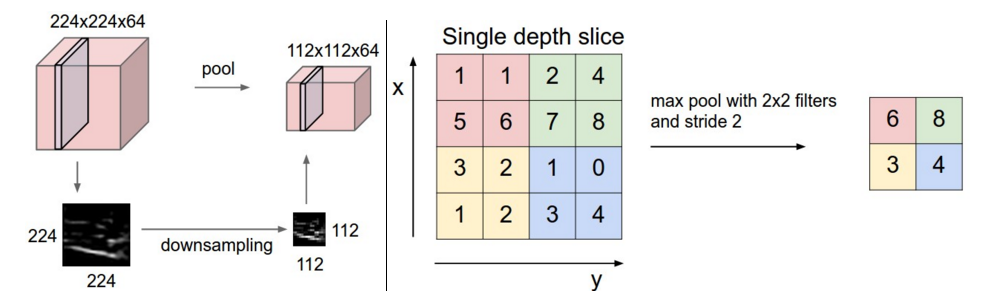
\includegraphics[scale=0.35]{pooling}
\end{frame}

\begin{frame}{Fully connected layers and dropout}
	\begin{itemize}
		\setlength\itemsep{1em}
		\setbeamertemplate{itemize item}[triangle]
		\setbeamercolor{itemize item}{fg=red}
		\item 
			Fully connected layers are the last layer of the CNN.
		\item 
			Once the high-level features are recognized, they deal with classifications.
		\item
			Dropout regolarization.
	\end{itemize}
	\begin{center}
		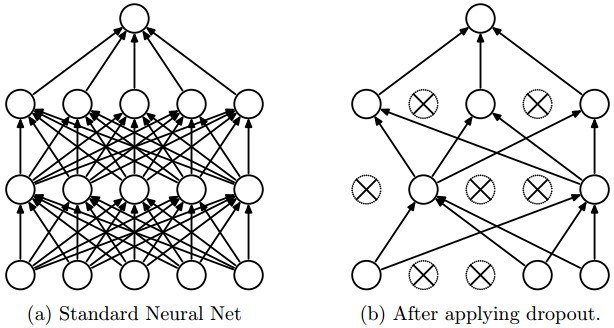
\includegraphics[scale=0.35]{dropout}
	\end{center}
\end{frame}

\begin{frame}{Activation functions}
	\begin{itemize}
		\setlength\itemsep{1em}
		\setbeamertemplate{itemize item}[triangle]
		\setbeamercolor{itemize item}{fg=red}
		\item 
			ReLU:
	\end{itemize}
	\begin{center}
		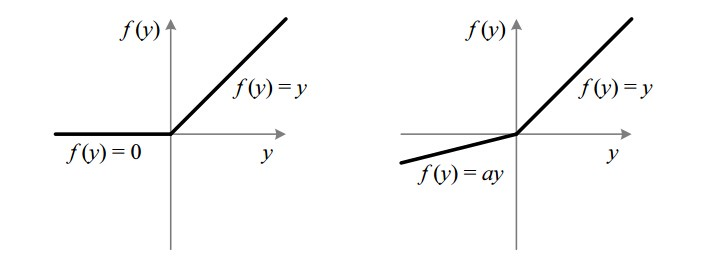
\includegraphics[scale=0.30]{ReLU}
	\end{center}
	\begin{itemize}
		\setlength\itemsep{1em}
		\setbeamertemplate{itemize item}[triangle]
		\setbeamercolor{itemize item}{fg=red}
		\item 
			Softmax (sigmoid and generical softmax):
	\end{itemize}
	\begin{center}
		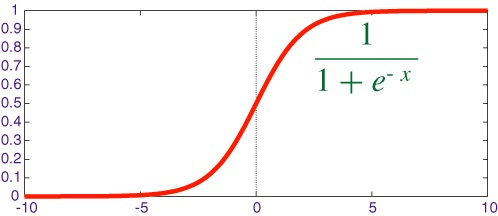
\includegraphics[scale=0.25]{softmax1}
		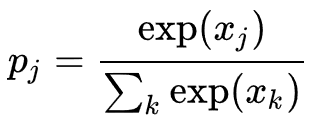
\includegraphics[scale=0.6]{softm}
	\end{center}
\end{frame}

\subsection{Dataset}

\begin{frame}{Dataset}
	\begin{itemize}
		\setlength\itemsep{1em}
		\setbeamertemplate{itemize item}[triangle]
		\setbeamercolor{itemize item}{fg=red}
		\item 
			The perfect dataset should be:
			\begin{itemize}
				\setbeamertemplate{itemize subitem}[circle]
				\setbeamercolor{itemize subitem}{fg=red}
				\item 
					made with thousands of images;
				\item 
					different images with different colors to help the network classify them better.
			\end{itemize}
	\end{itemize}
	\begin{center}
		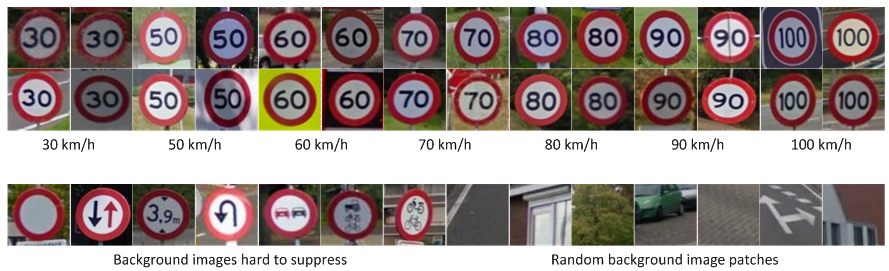
\includegraphics[scale=0.35]{datasets}
	\end{center}
\end{frame}

%\subsection{ImageNet}
%\begin{frame}{ImageNet Challenge}
%	\begin{itemize}
%		\setlength\itemsep{1em}
%		\setbeamertemplate{itemize item}[triangle]
%		\setbeamercolor{itemize item}{fg=red}
%		\item 
%			The ImageNet project:
%			\begin{itemize}
%				\setbeamertemplate{itemize subitem}[circle]
%				\setbeamercolor{itemize subitem}{fg=red}
%				\item 
%					large visual database designed for visual object recognition software research;
%				\item 
%					it contains over 20 thousand categories( "balloon", "strawberry", etc...);
%				\item
%					all the images are labelled.
%			\end{itemize}
%		\item 
%			ImageNet Large Scale Visual Recognition Challenge (ILSVRC):
%			\begin{itemize}
%				\setbeamertemplate{itemize subitem}[circle]
%				\setbeamercolor{itemize subitem}{fg=red}
%				\item 
%					is a competition where research teams evaluate their algorithms on the given data			%					set(ImageNet);
%				\item 
%					they compete to achieve higher accuracy on several visual recognition tasks.
%			\end{itemize}
%	\end{itemize}
%\end{frame}

\subsection{Inception V3 by Google}

\begin{frame}{Inception network (V3 - Example)}
	\begin{itemize}
		\setlength\itemsep{1em}
		\setbeamertemplate{itemize item}[triangle]
		\setbeamercolor{itemize item}{fg=red}
		\item 
			Inception network analizes images with different kernel size (in the same convolutional layer)
	\end{itemize}
	\begin{center}
		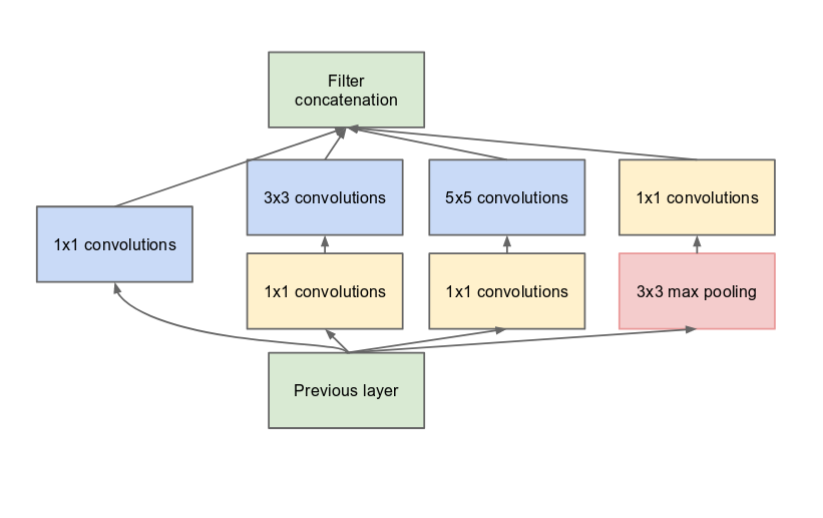
\includegraphics[scale=0.35]{inception}
	\end{center}
	%\begin{itemize}
		%\setlength\itemsep{1em}
		%\setbeamertemplate{itemize item}[triangle]
		%\setbeamercolor{itemize item}{fg=red}
		%\item 
			%Here an example: \href{https://bit.ly/2vBgoO3}{\color{red}GoogleNet}
	%\end{itemize}
\end{frame}

\subsection{Tensorflow and retraining}

\begin{frame}{Tensorflow and retraining}
	\begin{itemize}
		\setlength\itemsep{1em}
		\setbeamertemplate{itemize item}[triangle]
		\setbeamercolor{itemize item}{fg=red}
		\item 
			Concept of transfer learning (or retraining):  taking a piece of a model that has already been trained on a related task and reusing it in a new model.
		\item 
			Tensorflow-hub: the key to create your own classifier with good result and without a Tesla k80.
	\end{itemize}
\end{frame}
%#####################################PROPOSAL############################################################

\section{Proposed program}

\subsection{My work}

\begin{frame}
inserisci immagine divisa in tre con i tre "momenti"
\end{frame}

\subsection{Obtain images}

\begin{frame}{Obtain images}
	\begin{itemize}
		\setlength\itemsep{1em}
		\setbeamertemplate{itemize item}[triangle]
		\setbeamercolor{itemize item}{fg=red}

			\item 
				It uses OpenCv functions to get hundreds of photos in less than 30 seconds.
			\item 
				It crops photos by keeping only the faces(using haarcascadeclassifier) and it saves them.
			\item
				This is made to avoid the recognition of unwanted features as background color without 							the need of several images taken in different places.
		
	\end{itemize}
\end{frame}

\subsection{Retraining}

\begin{frame}{Training}
\begin{itemize}
		\setlength\itemsep{1em}
		\setbeamertemplate{itemize item}[triangle]
		\setbeamercolor{itemize item}{fg=red}
		
			\item 
				The algorithm takes the cropped images and use them as dataset for the training.
			\item 
				Only the fully connected layers are trained.
			\item
				More than 10x faster than a complete training.
		
	\end{itemize}
\end{frame}

\subsection{Inference}
\begin{frame}{Inference}
\begin{itemize}
		\setlength\itemsep{1em}
		\setbeamertemplate{itemize item}[triangle]
		\setbeamercolor{itemize item}{fg=red}
		
			\item 
				Choose a photo with multiple faces that you want to recognize/classify.
			\item 
				Select the already trained network you want to use for inference.
			\item
				Obtain the original photo with multiple boxes around all the faces and, under each of them, the name of the most probable person.
		
	\end{itemize}
\end{frame}



%#####################################SUMMARY############################################################

\section{Summary}

\subsection{Conclusion}
\begin{frame}{Conclusion}
	\begin{itemize}
	\setlength\itemsep{1em}
	\setbeamertemplate{itemize item}[triangle]
	\setbeamercolor{itemize item}{fg=red}
	\item 
		Creating your own machine learning application using another pre-trained model can help you build 					something useful without the need of high performance cluster or cloud computing.
	\item 
		The project, albeit simple, shows the potential of using Tensorflow and machine learning approaches in applications.
	\item
		Future works:
	\begin{itemize}
				\setbeamertemplate{itemize subitem}[circle]
				\setbeamercolor{itemize subitem}{fg=red}
    				\item
      					let the users choose beetwen more pre-trained models;
    				\item    
      					find the best way to recognize an unknown person (i.e. new student branch members).
 
			\end{itemize}
		
	\end{itemize}
\end{frame}

\begin{frame}{Best bugs}
	\begin{itemize}
		\setlength\itemsep{1em}
		\setbeamertemplate{itemize item}[triangle]
		\setbeamercolor{itemize item}{fg=red}
		\item 
			OpenCv \texttt{imshow} freezing bug on unix like system.
		\item 
			Tensorflow-hub requires a tensorflow version that could not work with some 								processors(precompiled with AVX activation)
			(\href{https://github.com/tensorflow/tensorflow/issues/17411}{\color{red}Link to issue}).
	\end{itemize}
\end{frame}

\appendix
\section<presentation>*{\appendixname}
\subsection<presentation>*{Useful links}

\begin{frame}{Useful links}
	\begin{itemize}
		\setlength\itemsep{1em}
		\setbeamertemplate{itemize item}[triangle]
		\setbeamercolor{itemize item}{fg=red}
		\item 
			Project repository: \href{https://github.com/SimoneCaldarella/faceRecognition}{\color{red}Link to repo}.
		\item 
			Tensorflow: \href{https://www.tensorflow.org}{\color{red}Link to Tensorflow page}.
		\item 
			OpenCv: \href{https://opencv.org}{\color{red}Link to OpenCv project}.
		\item 
			Convolutional Neural Network example: \href{https://bit.ly/2vBgoO3}{\color{red}GoogleNet}.
		\item 
			Tensorflow retrain: \href{https://www.tensorflow.org/hub/tutorials/image_retraining}{\color{red}tensorflow retraining}.
	\end{itemize}
\end{frame}

\end{document}


